\documentclass[
11pt, % The default document font size, options: 10pt, 11pt, 12pt
codirector, % Uncomment to add a codirector to the title page
]{charter} 


% El títulos de la memoria, se usa en la carátula y se puede usar el cualquier lugar del documento con el comando \ttitle
\titulo{Predicción de eventos climáticos y meteorológicos extremos utilizando inteligencia artificial} 

% Nombre del posgrado, se usa en la carátula y se puede usar el cualquier lugar del documento con el comando \degreename
%\posgrado{Carrera de Especialización en Sistemas Embebidos} 
%\posgrado{Carrera de Especialización en Internet de las Cosas} 
\posgrado{Carrera de Especialización en Inteligencia Artificial}
%\posgrado{Maestría en Sistemas Embebidos} 
%\posgrado{Maestría en Internet de las cosas}
% IMPORTANTE: no omitir titulaciones ni tildación en los nombres, también se recomienda escribir los nombres completos (tal cual los tienen en su documento)
% Tu nombre, se puede usar el cualquier lugar del documento con el comando \authorname
\autor{Ing. Sevann Radhak Triztan}

% El nombre del director y co-director, se puede usar el cualquier lugar del documento con el comando \supname y \cosupname y \pertesupname y \pertecosupname
\director{Título y Nombre del director}
\pertenenciaDirector{pertenencia} 
\codirector{Título y Nombre del codirector} % para que aparezca en la portada se debe descomentar la opción codirector en los parámetros de documentclass
\pertenenciaCoDirector{FIUBA}

% Nombre del cliente, quien va a aprobar los resultados del proyecto, se puede usar con el comando \clientename y \empclientename

\cliente{Carlos Roberto Salinas}
\empresaCliente{Dirección de Meteorología e Hidrología}
 
\fechaINICIO{18 de junio de 2024}		%Fecha de inicio de la cursada de GdP \fechaInicioName
\fechaFINALPlan{13 de agosto de 2024} 	%Fecha de final de cursada de GdP
\fechaFINALTrabajo{17 de diciembre de 2024}	%Fecha de defensa pública del trabajo final


\begin{document}

\maketitle
\thispagestyle{empty}
\pagebreak


\thispagestyle{empty}
{\setlength{\parskip}{0pt}
\tableofcontents{}
}
\pagebreak


\section*{Registros de cambios}
\label{sec:registro}


\begin{table}[ht]
\label{tab:registro}
\centering
\begin{tabularx}{\linewidth}{@{}|c|X|c|@{}}
\hline
\rowcolor[HTML]{C0C0C0} 
Revisión & \multicolumn{1}{c|}{\cellcolor[HTML]{C0C0C0}Detalles de los cambios realizados} & Fecha      \\ \hline
0      & Creación del documento                                 &\fechaInicioName \\ \hline
1      & Se completa hasta el punto 5 inclusive                & 2 de julio de 2024 \\ \hline
2      & Se completa hasta el punto 9 inclusive				 & 9 de julio de 2024 \\ \hline
%		  Se puede agregar algo más \newline
%		  En distintas líneas \newline
%		  Así                                                    & {día} de {mes} de 202X \\ \hline
%3      & Se completa hasta el punto 12 inclusive                & {día} de {mes} de 202X \\ \hline
%4      & Se completa el plan	                                 & {día} de {mes} de 202X \\ \hline

% Si hay más correcciones pasada la versión 4 también se deben especificar acá

\end{tabularx}
\end{table}

\pagebreak



\section*{Acta de constitución del proyecto}
\label{sec:acta}

\begin{flushright}
Buenos Aires, \fechaInicioName
\end{flushright}

\vspace{2cm}

Por medio de la presente se acuerda con el \authorname\hspace{1px} que su Trabajo Final de la \degreename\hspace{1px} se titulará ``\ttitle'' y consistirá esencialmente en la implementación de técnicas de inteligencia artificial (IA) para mejorar las predicciones de eventos climáticos y meteorológicos extremos. El trabajo tendrá un presupuesto preliminar estimado de 600 horas y un costo estimado de \textcolor{red}{\$ XXX}, con fecha de inicio el \fechaInicioName\hspace{1px} y fecha de presentación pública el \fechaFinalName.

Se adjunta a esta acta la planificación inicial.

\vfill

% Esta parte se construye sola con la información que hayan cargado en el preámbulo del documento y no debe modificarla
\begin{table}[ht]
\centering
\begin{tabular}{ccc}
\begin{tabular}[c]{@{}c@{}}Dr. Ing. Ariel Lutenberg \\ Director posgrado FIUBA\end{tabular} & \hspace{2cm} & \begin{tabular}[c]{@{}c@{}}\clientename \\ \empclientename \end{tabular} \vspace{2.5cm} \\ 
\multicolumn{3}{c}{\begin{tabular}[c]{@{}c@{}} \supname \\ Director del Trabajo Final\end{tabular}} \vspace{2.5cm} \\
\end{tabular}
\end{table}


\section{1. Descripción técnica-conceptual del proyecto a realizar}
\label{sec:descripcion}

El cambio climático y los eventos meteorológicos extremos presentan desafíos críticos a nivel global y local, afectando la vida, la infraestructura y la economía. En Paraguay, los eventos extremos como olas de calor, sequías y precipitaciones intensas han aumentado, destacando la necesidad urgente de mejorar la precisión y la efectividad de los pronósticos meteorológicos. 

Las actuales técnicas de monitoreo y predicción no siempre resultan suficientes para emitir advertencias tempranas y precisas. Este proyecto enfrenta el reto de adquirir, analizar y aplicar conocimientos para resolver problemas climatológicos complejos y busca utilizar la inteligencia artificial (IA) para analizar grandes volúmenes de datos meteorológicos y climáticos, tanto actuales como históricos, con el fin de mejorar la precisión de las predicciones y la toma de decisiones.

Este proyecto, propuesto por la \empclientename\hspace{1px} (DINAC) y el Parque Tecnológico Itaipu de Paraguay, busca abordar los desafíos actuales en la predicción de eventos climáticos extremos mediante el uso de herramientas de IA, contribuyendo así a mitigar los impactos del cambio climático en Paraguay y la región.

En la figura \ref{fig:diagBloques} se presenta el diagrama en bloques del sistema. Se observan los pasos propuestos para el desarrollo del presente proyecto. 

\begin{figure}[htpb]
\centering 
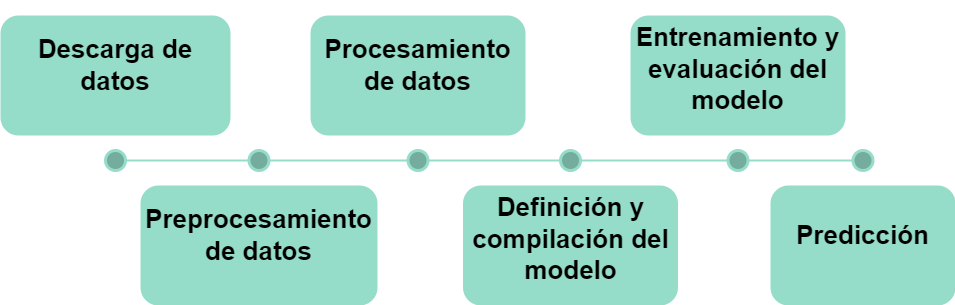
\includegraphics[width=.65\textwidth]{./Figuras/diagBloques.png}
\caption{Diagrama en bloques del sistema.}
\label{fig:diagBloques}
\end{figure}

\textbf{Descarga de datos:}
la \empclientename\hspace{1px} pondrá a disposición una base de datos para la obtención de datos históricos y actuales de las condiciones meteorológicas.

\textbf{Preprocesamiento de datos:}
se llevará a cabo un análisis de datos en crudo con el objetivo de dar tratamiento a datos vacíos, inconsistentes o conflictivos.

\textbf{Procesamiento de datos:}
serán aplicadas técnicas como la imputación de valores faltantes, reducción de dimensionalidad, estimación e interpretación de valores representativos, entre otras.

\textbf{Definición y compilación del modelo:}
diferentes modelos y técnicas serán propuestas, entrenadas y valuadas para comparar determinar el mejor modelo a utilizar.

\textbf{Entrenamiento y evaluación del modelo:}
el modelo seleccionado será entrenado con los datos procesados y evaluado aplicando técnicas avanzadas y métricas específicas para determinar su precisión y robustez.

\textbf{Predicción:}
una vez evaluado y ajustado el modelo, se procederá a realizar predicciones sobre los datos meteorológicos futuros, proporcionando información crítica para la toma de decisiones en la gestión de eventos climáticos extremos.


\vspace{25px}

\section{2. Identificación y análisis de los interesados}
\label{sec:interesados}

\begin{table}[ht]
%\caption{Identificación de los interesados}
%\label{tab:interesados}
\begin{tabularx}{\linewidth}{@{}|l|X|X|l|@{}}
\hline
\rowcolor[HTML]{C0C0C0} 
Rol           & Nombre y Apellido & Organización 	& Puesto 	\\ \hline
Cliente       & \clientename      &\empclientename	&   Gerente de Climatología     	\\ \hline
Product Owner       & \clientename      &\empclientename	&   Gerente de Climatología     	\\ \hline
Responsable   & \authorname       & FIUBA        	& Alumno 	\\ \hline
Orientador    & \supname	      & \pertesupname 	& Director del Trabajo Final \\ \hline
Usuario final & Sidney da Silva Viana                  & Central Hidroeléctrica Itaipu             	& Gerente de tecnologías en SI        	\\ \hline
\end{tabularx}
\end{table}

\begin{itemize}
	\item Cliente: el Dr. Ing. Sidney da Silva Vianna es experto en la temática, ejerce como Gerente de tecnologías en Sistemas de la Información (SI) y va a ayudar con la definición de los requerimientos y el desarrollo de la solución.
	\item Usuario final: Carlos Roberto Salinas, ejerce como 	Gerente de Climatología en la Dirección de Meteorología e Hidrología y la Dirección Nacional de Aeronáutica Civil. Nos proporcionara información útil respecto a las expectativas reales del usuario.
\end{itemize}

\section{3. Propósito del proyecto}
\label{sec:proposito}

Desarrollar un sistema avanzado de predicción de eventos climáticos y meteorológicos extremos utilizando técnicas de IA. Este sistema tiene como objetivo principal mejorar la precisión y la rapidez de los pronósticos meteorológicos, facilitando una respuesta más efectiva ante los fenómenos climáticos adversos y contribuyendo a la migración de sus impactos en Paraguay y sus alrededores.

\section{4. Alcance del proyecto}
\label{sec:alcance}

El proyecto incluye:
\begin{itemize}
	\item Recolección y preprocesamiento de datos:
		\begin{itemize}
		\item Obtención de datos meteorológicos históricos y actuales almacenados en la base de
datos de la DINAC.
		\item Limpieza, normalización y preprocesamiento de los datos para su uso en los modelos de IA.
		\end{itemize}
	\item Investigación y desarrollo de algoritmos de IA:
		\begin{itemize}
		\item Identificación y selección de algoritmos de IA adecuados para el análisis de datos meteorológicos.
		\item Desarrollo y ajuste de modelos de IA para predicción climática a corto y largo plazo.
		\end{itemize}
	\item Implementación de la Plataforma de predicción:
		\begin{itemize}
		\item Diseño y desarrollo de una plataforma tecnológica que integre los modelos de IA desarrollados.
		\item Implementación de interfaces de usuario para la visualización de predicciones y alertas.
		\end{itemize}
	\item Validación y optimización de modelos:
		\begin{itemize}
		\item Pruebas y validación de los modelos de predicción utilizando datos históricos y actuales.
		\item Optimización continua de los modelos para mejorar su precisión y eficiencia.
		\end{itemize}
	\item Gestión y monitoreo del proyecto:
		\begin{itemize}
		\item Establecimiento de un cronograma detallado y seguimiento del progreso del proyecto.
		\item Gestión de riesgos y resolución de problemas durante el desarrollo del proyecto.
		\end{itemize}
	
\end{itemize}

El proyecto no incluye:
\begin{itemize}
	\item Implementación de infraestructura física:
		\begin{itemize}
		\item La construcción, instalación o conexión a estaciones meteorológicas no está incluida.
		\item La actualización o mejora de la infraestructura física existente de recopilación de datos meteorológicos no forma parte del alcance del proyecto.
		\end{itemize}
	\item Mantenimiento a largo plazo:
		\begin{itemize}
		\item El mantenimiento continuo de la plataforma y los sistemas desarrollados, después de la finalización del proyecto, no está incluido.
		\item No se llevará a cabo mantenimiento regular post-implementación.
		\end{itemize}
	\item Distribución y gestión de alertas:
		\begin{itemize}
		\item La implementación de sistemas de distribución masiva de alertas no está incluida.
		\end{itemize}
	\item Integración con sistemas externos:
		\begin{itemize}
		\item La integración completa con otros sistemas de gestión de emergencias o bases de datos externas fuera del ámbito meteorológico no se incluye.
		\item El alcance del proyecto no contempla la integración directa con sistemas externos.
		\end{itemize}

\end{itemize}

\section{5. Supuestos del proyecto}
\label{sec:supuestos}

Para el desarrollo del presente proyecto se supone que: 

\begin{itemize}
	\item Se tendrá acceso continuo a una fuente de datos provista por la DINAC.
	\item La DINAC cuenta con una infraestructura tecnológica adecuada que permitirá el correcto entrenamiento y despliegue de la solución.
	\item Se fijarán y desarrollarán reuniones periódicas con el cliente para abordar temas relacionados con el proyecto.
	\item Se mantendrá la relación mediante el programa de vinculación con la DINAC hasta finalizar el desarrollo del proyecto.
\end{itemize}

\section{6. Requerimientos}
\label{sec:requerimientos}

\begin{enumerate}
	\item Requerimientos funcionales:
		\begin{enumerate}
			\item El sistema debe ser capaz de recolectar datos meteorológicos históricos y actuales de la base de datos de la DINAC.
			\item El sistema debe implementar y entrenar múltiples modelos de IA para determinar su conveniencia en términos de precisión, eficiencia y robustez.
			\item El sistema debe superar a los modelos actuales en términos precisión.
			\item El sistema debe emitir advertencias tempranas basadas en las predicciones de eventos extremos.
		\end{enumerate}
	\item Requerimientos No funcionales:
		\begin {enumerate}
			\item La solución debe estar programada de forma modular para que el código de sus características funcionales pueda ser fácilmente reutilizado y/o escalado.
			\item El sistema debe ser capaz de procesar grandes volúmenes de datos sin degradar su rendimiento.
		\end{enumerate}
	\item Requerimientos de datos:
		\begin {enumerate}
			\item Los datos meteorológicos históricos y actuales deben estar disponibles en la base de datos de la DINAC.
			\item Deben definirse formatos estándar para la importación y exportación de datos.
		\end{enumerate}
	\item Requerimientos de documentación:
		\begin{enumerate}
			\item Debe crearse una documentación técnica del sistema, incluyendo su arquitectura, diseño y funcionamiento.
		\end{enumerate}
	\item Requerimientos de testing:
		\begin{enumerate}
			\item La efectividad de los modelos será acordada y evaluada en conjunto con el cliente.
		\end{enumerate}
\end{enumerate}

\section{7. Historias de usuarios (\textit{Product backlog})}
\label{sec:backlog}

\begin{enumerate}
\item Como Product Owner, quiero obtener datos meteorológicos históricos y actuales de la base de datos de la DINAC para realizar análisis precisos.

\textit{Story points}: 6 (complejidad: 2, dificultad: 2, incertidumbre: 2)

\item Como Product Owner, quiero limpiar y normalizar los datos meteorológicos para garantizar su calidad ante los modelos de IA que serán entrenados.

\textit{Story points}: 9 (complejidad: 3, dificultad: 3, incertidumbre: 3)

\item Como Product Owner, quiero aplicar técnicas de imputación de valores faltantes para manejar datos incompletos.

\textit{Story points}: 7 (complejidad: 3, dificultad: 2, incertidumbre: 2)

\item Como Product Owner, quiero utilizar modelos de IA para predecir eventos climáticos extremos y mejorar la precisión de las predicciones.

\textit{Story points}: 10 (complejidad: 4, dificultad: 3, incertidumbre: 3)

\item Como Usuario, quiero comparar los resultados obtenidos de lo modelos de IA entrenados con el modelo actual para seleccionar el más adecuado para nuestras necesidades.

\textit{Story points}: 9 (complejidad: 3, dificultad: 3, incertidumbre: 3)

\item Como Product Owner, quiero emitir alertas tempranas de eventos climáticos extremos para tomar decisiones informadas y mitigar impactos.

\textit{Story points}: 9 (complejidad: 3, dificultad: 3, incertidumbre: 3)
\end{enumerate}

\section{8. Entregables principales del proyecto}
\label{sec:entregables}

\begin{itemize}
	\item Documento de Especificación de Requerimientos.
	\item Modelos de IA entrenados y evaluados.
	\item Sistema de predicción implementado.
	\item Informe Final del Proyecto.
	\item Código fuente y recursos digitales.
	\item Memoria del trabajo final.
\end{itemize}

\section{9. Desglose del trabajo en tareas}
\label{sec:wbs}

\begin{enumerate}
\item Grupo de Tareas 1: Recolección y preprocesamiento de datos (150 h)
	\begin{enumerate}
	\item Tarea 1: Definir y establecer la conexión con la base de datos de la DINAC (20 h)
	\item Tarea 2: Desarrollar scripts para la extracción automática de datos históricos y actuales (20 h)
	\item Tarea 3: Validar la integridad y calidad de los datos recolectados (20 h)
	\item Tarea 4: Documentar el proceso de obtención de datos (10 h)
	\item Tarea 5: Limpieza y normalización de datos para eliminar valores atípicos y errores (40 h)
	\item Tarea 6: Aplicación de técnicas de imputación para manejar datos faltantes (40 h)
	\end{enumerate}
\item Grupo de Tareas 2: Desarrollo y Evaluación de Modelos de IA (200 h)
	\begin{enumerate}
	\item Tarea 7: Investigar y seleccionar algoritmos apropiados para el análisis de datos meteorológicos (30 h)
	\item Tarea 8: Implementar los modelos seleccionados en el entorno de desarrollo (50 h)
	\begin{enumerate}
	\item Subtarea 8.1: Configurar el entorno de desarrollo para la implementación de modelos (10 h)	
	\item Subtarea 8.2: Desarrollar el código base para el primer modelo de IA (20 h)
	\item Subtarea 8.3: Desarrollar el código base para el segundo modelo de IA (20 h)
	\end{enumerate}		
	\item Tarea 9: Entrenar y ajustar los modelos con datos preprocesados (70 h)
	\begin{enumerate}
	\item Subtarea 9.1: Entrenar el primer modelo de IA con los datos preprocesados (20 h)
	\item Subtarea 9.2: Entrenar el segundo modelo de IA con los datos preprocesados (20 h)
	\item Subtarea 9.3: Realizar ajustes y optimizaciones en el primer modelo (15 h)
	\item Subtarea 9.4: Realizar ajustes y optimizaciones en el segundo modelo (15 h)
	\end{enumerate}	
	\item Tarea 10: Comparar la precisión y eficiencia de los modelos implementados con el modelo actual (50 h)
	\begin{enumerate}
	\item Subtarea 10.1: Definir métricas y criterios de evaluación para los modelos (10 h)
	\item Subtarea 10.2: Realizar pruebas de precisión y eficiencia en el primer modelo (20 h)
	\item Subtarea 10.3: Realizar pruebas de precisión y eficiencia en el segundo modelo (20 h)
	\end{enumerate}
	\end{enumerate}
\item Grupo de Tareas 3: Implementación del Sistema y Documentación (180 h)
\begin{enumerate}
	\item Tarea 11: Diseñar la arquitectura del sistema de predicción de eventos climáticos extremos (40 h)
	\item Tarea 12: Implementar el proceso de emisión de predicciones y alertas (40 h)
	\item Tarea 13: Integrar los modelos de IA con la plataforma desarrollada (40 h)
	\item Tarea 14: Elaborar la documentación técnica del sistema y los manuales de usuario (20 h)
	\item Realizar pruebas de aceptación con el cliente para validar la funcionalidad del sistema (40 h)
	\end{enumerate}
\item Tareas 4: Gestión del proyecto y presentación (70 h)
\begin{enumerate}
	\item Tarea 15: Gestionar riesgos y problemas durante el desarrollo del proyecto (40 h)
	\item Tarea 16: Preparar la presentación pública del proyecto y demostración ante el tribunal (30 h)
	\end{enumerate}
\end{enumerate}

Cantidad total de horas: 600 h.

\section{10. Diagrama de Activity On Node}
\label{sec:AoN}

\begin{consigna}{red}
Armar el AoN a partir del WBS definido en la etapa anterior.

Una herramienta simple para desarrollar los diagramas es el Draw.io (\url{https://app.diagrams.net/}).
\href{https://app.diagrams.net}{Draw.io}


\begin{figure}[htpb]
\centering 
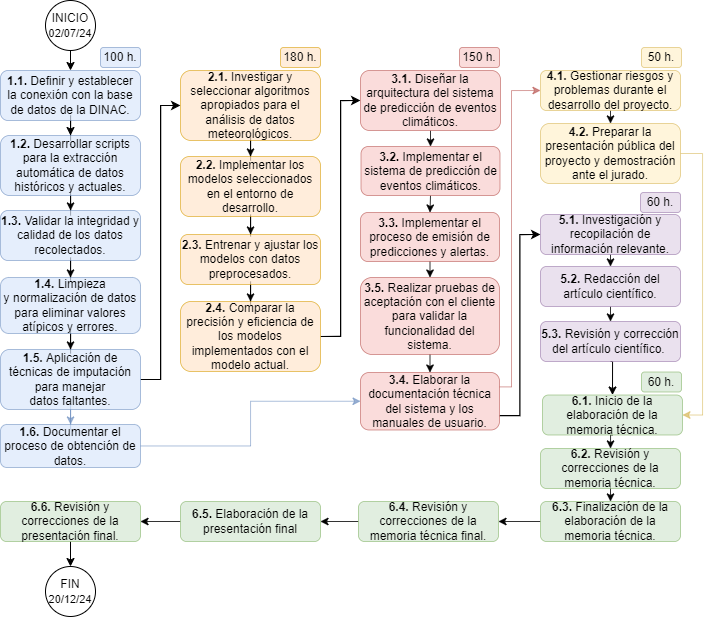
\includegraphics[width=.8\textwidth]{./Figuras/AoN.png}
\caption{Diagrama de \textit{Activity on Node}.}
\label{fig:AoN}
\end{figure}

Indicar claramente en qué unidades están expresados los tiempos.
De ser necesario indicar los caminos semi críticos y analizar sus tiempos mediante un cuadro.
Es recomendable usar colores y un cuadro indicativo describiendo qué representa cada color.

\end{consigna}

\section{11. Diagrama de Gantt}
\label{sec:gantt}

\begin{consigna}{red}
Existen muchos programas y recursos \textit{online} para hacer diagramas de Gantt, entre los cuales destacamos:

\begin{itemize}
\item Planner
\item GanttProject
\item Trello + \textit{plugins}. En el siguiente link hay un tutorial oficial: \\ \url{https://blog.trello.com/es/diagrama-de-gantt-de-un-proyecto}
\item Creately, herramienta online colaborativa. \\\url{https://creately.com/diagram/example/ieb3p3ml/LaTeX}
\item Se puede hacer en latex con el paquete \textit{pgfgantt}\\ \url{http://ctan.dcc.uchile.cl/graphics/pgf/contrib/pgfgantt/pgfgantt.pdf}
\end{itemize}

Pegar acá una captura de pantalla del diagrama de Gantt, cuidando que la letra sea suficientemente grande como para ser legible. 
Si el diagrama queda demasiado ancho, se puede pegar primero la ``tabla'' del Gantt y luego pegar la parte del diagrama de barras del diagrama de Gantt.

Configurar el software para que en la parte de la tabla muestre los códigos del EDT (WBS).\\
Configurar el software para que al lado de cada barra muestre el nombre de cada tarea.\\
Revisar que la fecha de finalización coincida con lo indicado en el Acta Constitutiva.

En la figura \ref{fig:gantt}, se muestra un ejemplo de diagrama de gantt realizado con el paquete de \textit{pgfgantt}. 
En la plantilla pueden ver el código que lo genera y usarlo de base para construir el propio.

Las fechas pueden ser calculadas utilizando alguna de las herramientas antes citadas. Sin embargo, el siguiente ejemplo
fue elaborado utilizando 
\href{https://docs.google.com/spreadsheets/d/1fBz8NhSpc4tkkhz3KjJCbh1nR_ltDkfEcZi4tZXduqs}{esta hoja de cálculo}.

Es importante destacar que el ancho del diagrama estará dado por la longitud del texto utilizado para las tareas 
(Ejemplo: tarea 1, tarea 2, etcétera) y el valor \textit{x unit}. Para mejorar la apariencia del diagrama, es necesario
ajustar este valor y, quizás, acortar los nombres de las tareas.

\begin{figure}[htpb]
  \begin{center}
    \begin{ganttchart}[
      time slot unit=day,
      time slot format=isodate,
      x unit=0.038cm,
      y unit title=0.7cm,
      y unit chart=0.6cm,
      milestone/.append style={xscale=4}
      ]{2021-03-05}{2021-12-16}
      \gantttitlecalendar*{2021-03-05}{2021-12-16}{year} \\
      \gantttitlecalendar*{2021-03-05}{2021-12-16}{month} \\
      \ganttgroup{Duración Total}{2021-03-05}{2021-12-16} \\
      %%%%%%%%%%%%%%%%%Organización
      \ganttgroup{Organización}{2021-03-05}{2021-04-16} \\
      \ganttbar{Planificación del proyecto}{2021-03-05}{2021-04-15} \\
      %%%%%%%%%%%%%%%%%Ejecución
      \ganttgroup{Ejecución}{2021-04-16}{2021-10-21} \\
      \ganttbar{Tarea 1}{2021-04-16}{2021-04-29} \\
      \ganttbar{Tarea 2}{2021-04-30}{2021-05-13} \\
      \ganttbar{Tarea 3}{2021-05-14}{2021-05-27} \\
      \ganttbar{Tarea 4}{2021-05-28}{2021-07-12} \\
      \ganttbar{Tarea 5}{2021-07-13}{2021-08-09} \\
      \ganttbar{Tarea 6}{2021-08-10}{2021-09-23} \\
      \ganttbar{Tarea 7}{2021-09-24}{2021-09-30} \\
      \ganttbar{Tarea 8}{2021-10-01}{2021-10-14} \\
      \ganttbar{Tarea 9}{2021-10-15}{2021-10-21} \\
      % %%%%%%%%%%%%%%%%%Finalización
      \ganttgroup{Finalización}{2021-10-22}{2021-12-16} \\
      \ganttbar{Memoria v1}{2021-10-22}{2021-11-04} \\
      \ganttbar{Memoria v2}{2021-11-05}{2021-11-18} \\
      \ganttbar{Memoria final}{2021-11-19}{2021-12-02} \\
      % La fecha del siguiente milestone es la fecha en que terminamos la memoria
      \ganttmilestone{Enviar memoria al director}{2021-12-02} \\
      \ganttbar{Elaborar la presentación}{2021-12-03}{2021-12-16} \\
      \ganttmilestone{Ensayo de la presentación}{2021-12-16} \\
      %%%%%%%%%%%%%%%%%%%%%%%%%%%%%%%%%%%%%%%%%%%%%%%%%%%%%%%%%%%%%%%
    \end{ganttchart}
  \end{center}
  \caption{Diagrama de gantt de ejemplo}
  \label{fig:gantt}
\end{figure}


\begin{landscape}
\begin{figure}[htpb]
\centering 
\includegraphics[height=.85\textheight]{./Figuras/Gantt-2.png}
\caption{Ejemplo de diagrama de Gantt (apaisado).} %Modificar este título acorde.
\label{fig:diagGantt}
\end{figure}

\end{landscape}

\end{consigna}


\section{12. Presupuesto detallado del proyecto}
\label{sec:presupuesto}

\begin{consigna}{red}
Si el proyecto es complejo entonces separarlo en partes:
\begin{itemize}
	\item Un total global, indicando el subtotal acumulado por cada una de las áreas.
	\item El desglose detallado del subtotal de cada una de las áreas.
\end{itemize}

IMPORTANTE: No olvidarse de considerar los COSTOS INDIRECTOS.

Incluir la aclaración de si se emplea como moneda el peso argentino (ARS) o si se usa moneda extranjera (USD, EUR, etc). Si es en moneda extranjera se debe indicar la tasa de conversión respecto a la moneda local en una fecha dada.

\end{consigna}

\begin{table}[htpb]
\centering
\begin{tabularx}{\linewidth}{@{}|X|c|r|r|@{}}
\hline
\rowcolor[HTML]{C0C0C0} 
\multicolumn{4}{|c|}{\cellcolor[HTML]{C0C0C0}COSTOS DIRECTOS} \\ \hline
\rowcolor[HTML]{C0C0C0} 
Descripción &
  \multicolumn{1}{c|}{\cellcolor[HTML]{C0C0C0}Cantidad} &
  \multicolumn{1}{c|}{\cellcolor[HTML]{C0C0C0}Valor unitario} &
  \multicolumn{1}{c|}{\cellcolor[HTML]{C0C0C0}Valor total} \\ \hline
 &
  \multicolumn{1}{c|}{} &
  \multicolumn{1}{c|}{} &
  \multicolumn{1}{c|}{} \\ \hline
 &
  \multicolumn{1}{c|}{} &
  \multicolumn{1}{c|}{} &
  \multicolumn{1}{c|}{} \\ \hline
\multicolumn{1}{|l|}{} &
   &
   &
   \\ \hline
\multicolumn{1}{|l|}{} &
   &
   &
   \\ \hline
\multicolumn{3}{|c|}{SUBTOTAL} &
  \multicolumn{1}{c|}{} \\ \hline
\rowcolor[HTML]{C0C0C0} 
\multicolumn{4}{|c|}{\cellcolor[HTML]{C0C0C0}COSTOS INDIRECTOS} \\ \hline
\rowcolor[HTML]{C0C0C0} 
Descripción &
  \multicolumn{1}{c|}{\cellcolor[HTML]{C0C0C0}Cantidad} &
  \multicolumn{1}{c|}{\cellcolor[HTML]{C0C0C0}Valor unitario} &
  \multicolumn{1}{c|}{\cellcolor[HTML]{C0C0C0}Valor total} \\ \hline
\multicolumn{1}{|l|}{} &
   &
   &
   \\ \hline
\multicolumn{1}{|l|}{} &
   &
   &
   \\ \hline
\multicolumn{1}{|l|}{} &
   &
   &
   \\ \hline
\multicolumn{3}{|c|}{SUBTOTAL} &
  \multicolumn{1}{c|}{} \\ \hline
\rowcolor[HTML]{C0C0C0}
\multicolumn{3}{|c|}{TOTAL} &
   \\ \hline
\end{tabularx}%
\end{table}


\section{13. Gestión de riesgos}
\label{sec:riesgos}

\begin{consigna}{red}
a) Identificación de los riesgos (al menos cinco) y estimación de sus consecuencias:
 
Riesgo 1: detallar el riesgo (riesgo es algo que si ocurre altera los planes previstos de forma negativa)
\begin{itemize}
	\item Severidad (S): mientras más severo, más alto es el número (usar números del 1 al 10).\\
	Justificar el motivo por el cual se asigna determinado número de severidad (S).
	\item Probabilidad de ocurrencia (O): mientras más probable, más alto es el número (usar del 1 al 10).\\
	Justificar el motivo por el cual se asigna determinado número de (O). 
\end{itemize}   

Riesgo 2:
\begin{itemize}
	\item Severidad (S): X.\\
	Justificación...
	\item Ocurrencia (O): Y.\\
	Justificación...
\end{itemize}

Riesgo 3:
\begin{itemize}
	\item Severidad (S):  X.\\
	Justificación...
	\item Ocurrencia (O): Y.\\
	Justificación...
\end{itemize}


b) Tabla de gestión de riesgos:      (El RPN se calcula como RPN=SxO)

\begin{table}[htpb]
\centering
\begin{tabularx}{\linewidth}{@{}|X|c|c|c|c|c|c|@{}}
\hline
\rowcolor[HTML]{C0C0C0} 
Riesgo & S & O & RPN & S* & O* & RPN* \\ \hline
       &   &   &     &    &    &      \\ \hline
       &   &   &     &    &    &      \\ \hline
       &   &   &     &    &    &      \\ \hline
       &   &   &     &    &    &      \\ \hline
       &   &   &     &    &    &      \\ \hline
\end{tabularx}%
\end{table}

Criterio adoptado: 

Se tomarán medidas de mitigación en los riesgos cuyos números de RPN sean mayores a...

Nota: los valores marcados con (*) en la tabla corresponden luego de haber aplicado la mitigación.

c) Plan de mitigación de los riesgos que originalmente excedían el RPN máximo establecido:
 
Riesgo 1: plan de mitigación (si por el RPN fuera necesario elaborar un plan de mitigación).
  Nueva asignación de S y O, con su respectiva justificación:
  \begin{itemize}
	\item Severidad (S*): mientras más severo, más alto es el número (usar números del 1 al 10).
          Justificar el motivo por el cual se asigna determinado número de severidad (S).
	\item Probabilidad de ocurrencia (O*): mientras más probable, más alto es el número (usar del 1 al 10).
          Justificar el motivo por el cual se asigna determinado número de (O).
	\end{itemize}

Riesgo 2: plan de mitigación (si por el RPN fuera necesario elaborar un plan de mitigación).
 
Riesgo 3: plan de mitigación (si por el RPN fuera necesario elaborar un plan de mitigación).

\end{consigna}


\section{14. Gestión de la calidad}
\label{sec:calidad}

\begin{consigna}{red}
Elija al menos diez requerimientos que a su criterio sean los más importantes/críticos/que aportan más valor y para cada uno de ellos indique las acciones de verificación y validación que permitan asegurar su cumplimiento.

\begin{itemize} 
\item Req \#1: copiar acá el requerimiento con su correspondiente número.

\begin{itemize}
	\item Verificación para confirmar si se cumplió con lo requerido antes de mostrar el sistema al cliente. Detallar.
	\item Validación con el cliente para confirmar que está de acuerdo en que se cumplió con lo requerido. Detallar. 
\end{itemize}

\end{itemize}

Tener en cuenta que en este contexto se pueden mencionar simulaciones, cálculos, revisión de hojas de datos, consulta con expertos, mediciones, etc.  

Las acciones de verificación suelen considerar al entregable como ``caja blanca'', es decir se conoce en profundidad su funcionamiento interno.  

En cambio, las acciones de validación suelen considerar al entregable como ``caja negra'', es decir, que no se conocen los detalles de su funcionamiento interno.

\end{consigna}

\section{15. Procesos de cierre}    
\label{sec:cierre}

\begin{consigna}{red}
Establecer las pautas de trabajo para realizar una reunión final de evaluación del proyecto, tal que contemple las siguientes actividades:

\begin{itemize}
	\item Pautas de trabajo que se seguirán para analizar si se respetó el Plan de Proyecto original:\\
	 - Indicar quién se ocupará de hacer esto y cuál será el procedimiento a aplicar. 
	\item Identificación de las técnicas y procedimientos útiles e inútiles que se emplearon, los problemas que surgieron y cómo se solucionaron:\\
	 - Indicar quién se ocupará de hacer esto y cuál será el procedimiento para dejar registro.
	\item Indicar quién organizará el acto de agradecimiento a todos los interesados, y en especial al equipo de trabajo y colaboradores:\\
	  - Indicar esto y quién financiará los gastos correspondientes.
\end{itemize}

\end{consigna}

\end{document}